\section{Objectives Summarised}

\begin{enumerate}
    \item The program should be capable of procedurally drawing a road network to the UI.
    \item The number of vertices should be limited to 50 to prevent slowing down the simulation.
    \item The user should be able to save and load road networks in and out of the program.
    \item The program should support a click-and-drag based interaction, allowing the creation of vertices and connections and further editing of the network.
    \item The user should also be able to undo and redo actions to the road network.
    \item The program should be able to simulate cars driving sensibly across the road network.
    \item The maximum number of agents active at any time should be limited to 60.
    \item Relevant output data described in \autoref{analysis} should be outputted to both the UI and downloadable files.
    \item There should be a minimalist interface with the majority of screen real-estate allocated to the network visualisation.
    \item This program should support desktop size displays.
    \item It should also be compatible with variable aspect ratios, resizing UI elements to fit the screen.
\end{enumerate}

\section{Front-end}

    \subsection{Network construction}

        As shown in \autoref{testing:gui-screenshot}, I have developed a program that displays a 2D road network. Utilising a graph data structure on the back end along with cubic Bezier curves to allow for curving road sections.

        \begin{figure}
            \centering
            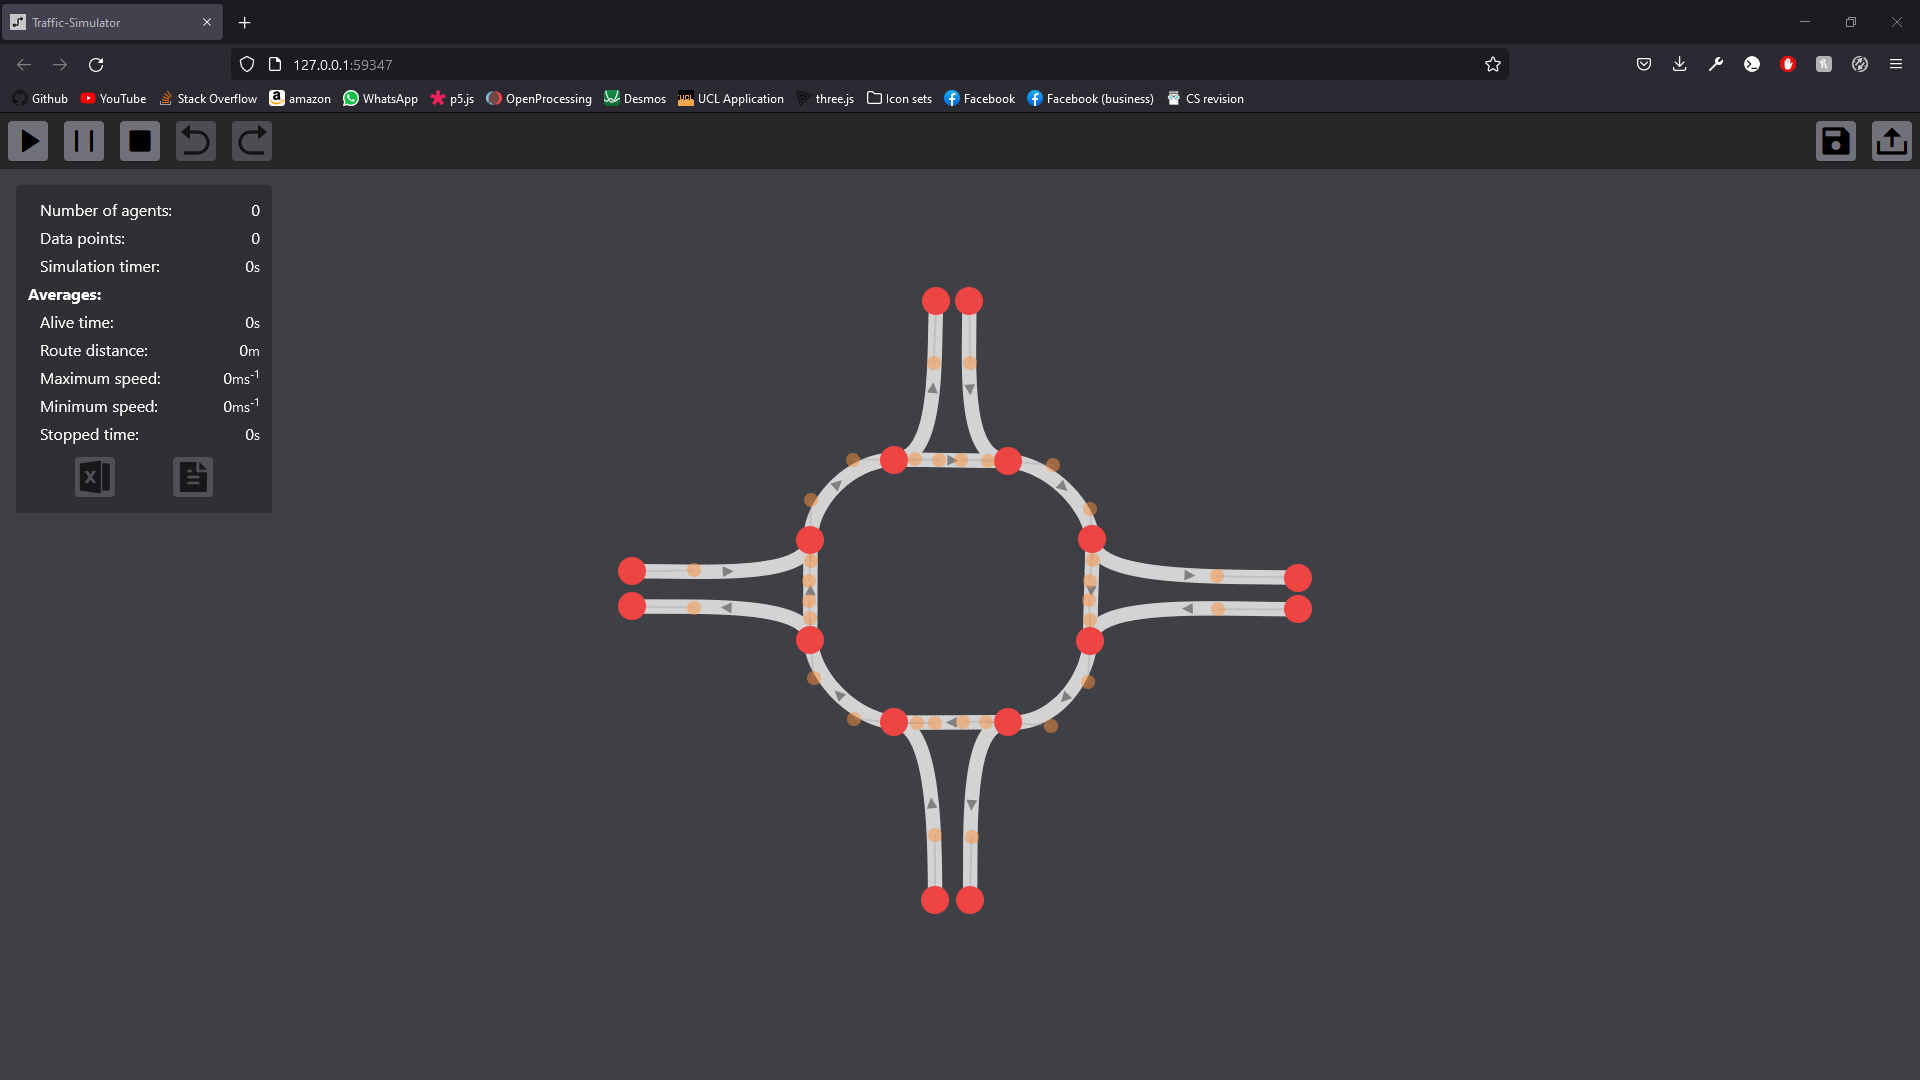
\includegraphics[width=0.6\textwidth]{gui-screenshot.png}
            \caption{Screenshot of final program}
            \label{testing:gui-screenshot}
        \end{figure}

        I have also implemented a mainly mouse-based graph editing system, allowing the user to manipulate and design their own road network. \autoref{testing:construction-examples} shows a few demo networks I have built using this program.


    \subsection{Videos}

        As part of the testing process for this project I have produced a video displaying the front-end user interaction. Making use of the majority of features I have implemented. Please note that the keyboard and mouse overlay are for clarity purposes only and not part of the program.

        \href{https://youtu.be/RnU7ZQtnQWU}{NEA testing video 1}

\section{Back-end}

    During the development process I wrote a series of unit tests to validate the major parts of the system, leading to less error-prone and maintainable code. The following index (\autoref{tests-index}) points to the test files in my code base. All the tests pass when executed.

    \begin{table}
        \begin{tabular}{|p{0.45\textwidth}|p{0.45\textwidth}|}
            \hline
            \textbf{Test target} & \textbf{Link}\\\hline
            Graph & \href{https://github.com/joshua-smart/traffic-simulator/blob/main/src/tests/model/graph.test.ts}{src/tests/model/graph.test.ts}\\\hline
            RoadNetwork & \href{https://github.com/joshua-smart/traffic-simulator/blob/main/src/tests/model/roadNetwork.test.ts}{src/tests/model/roadNetwork.test.ts}\\\hline
            Simulation & \href{https://github.com/joshua-smart/traffic-simulator/blob/main/src/tests/model/simulation.test.ts}{src/tests/model/simulation.test.ts}\\\hline
        \end{tabular}
        \caption{Unit tests index}
        \label{tests-index}
    \end{table}
